\documentclass[a4paper, twoside]{article}
\usepackage[utf8]{inputenc} % Especifica la codificación de caracteres de los documentos.
\usepackage[spanish]{babel} % Indica que el documento se escribirá en español.
\usepackage[top=3cm, bottom=2.5cm, inner=1.5cm, outer=2.5cm]{geometry} % Márgenes personalizados
\usepackage{subfiles} % Paquete para incluir el preambulo en los sub archivos.
\usepackage{afterpage} % Permite añadir páginas despues de una página dada.
\usepackage{hyperref} % Permite incluir enlaces en los archivos.
\usepackage{lastpage} % Paquete para poder contabilizar el total de páginas del documento.
\usepackage{fancyhdr} % Permite personalizar los header y footer del documento.
\usepackage{graphicx} % Permite incluir gráficos
\usepackage[hang, bf]{caption} % Personaliza los subtítulos de las figuras y tablas
\usepackage{float} % Permite posicionar mejor las figuras y tablas

% Defino la ruta de los paquetes personalizados para el apunte
\newcommand{\rutapaquetes}{./paquetes-apunte}

\usepackage[mostrarlicencia]{\rutapaquetes/caratula} % Caratula personalizada (cargada desde caratula.sty)
\usepackage[mostrarrevisores]{\rutapaquetes/colaboradores} % Seccion de colaboradores (cargada y creada con colaboradores.sty)
\usepackage{\rutapaquetes/historial} % Seccion de historial de cambios (cargada y creada con historial.sty)

% Define los estilos de los enlaces interpretados por el paquete hyperref
\hypersetup{
	colorlinks=true,   % false: boxed links; true: colored links
	linkcolor=black,   % color of internal links (change box color with linkbordercolor)
	citecolor=green,   % color of links to bibliography
	filecolor=magenta, % color of file links
	urlcolor=blue,     % color of external links
}

\newcommand{\imgdir}{../resources/images} % Ruta de las imágenes

% Define los directorios de las imágenes y gráficos
\graphicspath{ {\imgdir/} {\rutapaquetes/} }

\newcommand{\nombremateria}{Sistemas Operativos (75.08 - 95.03)} % Defino el comando "\nombremateria" para no harcodear el nombre en varios lugares.

% Define el pagestyle personalizado
\pagestyle{fancy}
\fancyhf{}
\renewcommand{\sectionmark}[1]{\markboth{}{\thesection\ \ #1}}
% Define header para pagina par
\fancyhead[ER]{\rightmark}
% Define header para pagina impar
\fancyhead[OL]{\rightmark}
% Define footer para pagina par
\fancyfoot[EL]{\nombremateria} % Nombre del apunte a la izquierda
\fancyfoot[ER]{Página \thepage\ de \pageref{LastPage}} % Numero de pagina a la derecha
% Define footer para pagina impar
\fancyfoot[OL]{Página \thepage\ de \pageref{LastPage}} % Numero de pagina a la izquierda
\fancyfoot[OR]{\nombremateria} % Nombre del apunte a la derecha

\renewcommand{\footrulewidth}{0.4pt} % Agrego linea que separa el footer

% Configura la caratula
\materia{\nombremateria}
\tipoapunte{Resumen teórico}
%\tema{Tema de la Materia}
%\subtema{Subtema}

\begin{document}
% Página en blanco agregada después de la carátula
%\afterpage{
%	\null
%	\thispagestyle{empty}%
%	\addtocounter{page}{-1}%
%	\newpage}
\maketitle % Genera la carátula

\tableofcontents % Genera el índice

\subfile{\rutapaquetes/acerca-del-proyecto.tex} % Inlcuye informacion acerca del proyecto FIUBA Apuntes

% Insertar aquí el contenido del apunte. A continuacion hay secciones a modo de ejemplo.

\section{Introducción}
\subsection{¿Qué es un sistema operativo?}
\begin{itemize}
	\item Un programa que hace de intermediario entre el usuario de la computadora y su hardware (Oculta los detalles finos de la arquitectura).
	\item Un programa que administra los recursos de un sistema de computación: permite administrar el tiempo de procesador y el espacio (memoria, disco, etc).
\end{itemize}

\subsection{Arquitecturas}
\subsubsection{Mainframe}
Computadora central. Gran capacidad de I/O, server para e-commerce a gran escala.\\

\textbf{Seguridad y disponibilidad:} 
\begin{itemize}
	\item Transaction processing: is information processing that is divided into individual, indivisible operations, called transactions. Each transaction must succeed or fail as a complete unit; it can never be only partially complete.
	\item Batch processing: is the execution of a series of programs ("jobs") on a computer without manual intervention.
\end{itemize}

\subsubsection{Servidores}
Destinados a ofrecer servicios a través de una red.

\subsubsection{Supercomputadoras}
Computacion de alto rendimiento. Se usan para hacer simulaciones.\\

\textbf{Limites:}
\begin{itemize}
	\item Concurrencia: los procesos no son 100\% independientes
	\item Costo
	\item Programación del software
\end{itemize}

\subsubsection{Server operating system}
Interfaz solo línea de comando o EFI (estándar de firmware).

\subsubsection{Computadora personal}
No requiere conocimientos especiales.

\subsubsection{Tablets, PDA}

\subsubsection{Consolas}

\subsubsection{Sistemas operativos embebidos}
Dispositivos que no aceptan instalación de nuevo software por el usuario.

No deberían tener bugs.

Se usan en tvs, autos, etc.

\subsubsection{Cluster}
Un grupo de computadoras interconectadas por una red local de alta velocidad.

Se comportan como si fuese una única computadora.

Si es de alta disponibilidad tiene nodos redundantes en caso de falla. Retoma en otro equipo en el estado en el que estaba. 

Balance de carga, con dispositivo físico o de software.

\subsubsection{Grid}
Cluster virtual con recursos distribuidos.

\textbf{Ejemplo:} BOINC, SETI.

\textbf{Problemas:} concurrencia (que se choquen tareas), que queden tareas sin cubrir.

\subsubsection{Cloud computing}
Se provee por internet. Dinamicamente escalable.

Atrás de la nube puede haber cluster, grid, etc (al cliente no le importa).

\textbf{Servicios posibles de cloud computing:}
\begin{itemize}
	\item Cloud Storage: Dropbox.
	\item Infraestructura (infraestructura as a service (IaaS)):Tipicamente plataformas virtualizadas. Ejemplo: Amazon EC2
	\item Plataforma (PaaS): Provee la plataforma y un ambiente de desarrollo y soporte. Ejemplo: Google Code.
	\item Software (SaaS): Software on demand provisto por terceros. Ejemplo: Amazon Services, Paypal. 
\end{itemize}

\subsubsection{Tiempo real}
Distinto de online o de rápido.

Tiempo de respuesta máximo y predecible. 

\subsubsection{Multiprocesador}
Más de un procesador en el mismo chip o board.

Soportado en todos los sistemas operativos de escritorio.

La paralelizacion esta limitada por la ley de Amdahl: The speedup of a program using multiple processors in parallel computing is limited by the time needed for the sequential fraction of the program.

\newpage
\section{Mecanismos básicos}
Sistema operativo es software que extiende un poco la capa de hardware.

El hardware es lo que le provee recursos al sistema operativo: CPU, memoria, dispositivos I/O. Cada nivel interpreta al nivel superior.

El estado de una maquina virtual sólo está definido entre instrucción e instrucción.

Una instrucción en una capa equivale a muchas instrucciones de la capa inferior.

\subsection{Modos de CPU}
Son distintos niveles de permisos o privilegios.

Se suele trabajar con dos modos: \textbf{Modo Supervisor} (puede hacer todo) y \textbf{Modo Usuario} (tiene restricciones).

Se pasa de modo usuario a modo supervisor por medio de una interrupción. 

El retorno a modo usuario está a cargo del programa. Motivo para querer pasar de modo supervisor a modo usuario: Control de riesgo de código desconocido (ejemplo: escribir en las direcciones de memoria del SO).\\

Algunas arquitecturas incluyen más modos:
\begin{itemize}
	\item X86 Modo real, protegido y virtual.
	\item Modo hypervisor
\end{itemize}

Un sistema operativo puede tener partes corriendo en cada uno de los modos.

Un programa de usuario sólo corre en modo usuario. El único programa que debiera ser capaz de pasar a modo supervisor es el sistema operativo.

\subsection{Interrupciones}
Una interrupción es una suspensión temporal de la ejecución de un proceso, para pasar a ejecutar una subrutina de servicio de interrupción, la cual, por lo general, no forma parte del programa, sino que pertenece al sistema operativo o al BIOS. Una vez finalizada dicha subrutina, se reanuda la ejecución del programa.\\

Hay dos tipos de interrupciones:
\begin{itemize}
	\item Sincronica o software trap: Una instrucción del programa.
	\item Asincrónica: I/O, timer, external.
\end{itemize}

\subsubsection{Atención de interrupciones}
\begin{enumerate}
	\item \textbf{Primer nivel de atención:} Salvar el contexto (registros, código de condición, dirección de retorno). El objetivo es poder proseguir el proceso (después de atendida la interrupción) desde el estado en el que estaba. Que un proceso sufra o no una interrupción no cambia su resultado, solamente el tiempo que le insume.
	
	\item \textbf{Segundo nivel de atención:} Se decide si se atiende en el momento la interrupción o se deja para después. Si vienen 2 interrupciones al mismo tiempo puede llegar a perderse una. Por eso los que envían la interrupción deben estar preparados para repetirla.
\end{enumerate}

\subsection{Modos del sistema operativo}
\subsubsection{Modo Kernel}
Ejecutando un servicio propio del sistema operativo.

In computing, the kernel is a computer program that manages input/output requests from software, and translates them into data processing instructions for the central processing unit and other electronic components of a computer. The kernel is a fundamental part of a modern computer's operating system.

Because of its critical nature, the kernel code is usually loaded into a protected area of memory, which prevents it from being overwritten by other, less frequently used parts of the operating system or by application programs. The kernel performs its tasks, such as executing processes and handling interrupts, in kernel space, whereas everything a user normally does, such as writing text in a text editor or running programs in a GUI (graphical user interface), is done in user space. This separation is made in order to prevent user data and kernel data from interfering with each other and thereby diminishing performance or causing the system to become unstable (and possibly crashing).

When a computer program (in this context called a process) makes requests of the kernel, the request is called a system call.

\subsubsection{Modo usuario}
Ejecutando un programa de usuario.

The term userland (or user space) refers to all code which runs outside the operating system's kernel. Userland usually refers to the various programs and libraries that the operating system uses to interact with the kernel: software that performs input/output, manipulates file system objects, application software etc.

\subsection{System Calls}
Si un proceso esta corriendo un programa en modo usuario y necesita un servicio del sistema, como leer data de un archivo, tiene que ejecutar un software trap para transferirle el control al sistema operativo. El sistema operativo se fija lo que necesita el proceso que lo  llamo inspeccionando los parámetros. Hace lo que tenga que hacer y devuelve el control a la instrucción que sigue al system call.\\

Ejemplos
\begin{itemize}
	\item Leer de un dispositivo solo puede hacer el SO (leer de memoria, CD, USB, etc).
	\item Manejo de procesos
	\item Manejo de archivos
	\item Etc
\end{itemize}

\subsection{Library Calls}
Son llamados a procedimientos de bibliotecas provistas por el lenguaje en el que se está programando.\\

\begin{figure}[H]
	\centering
	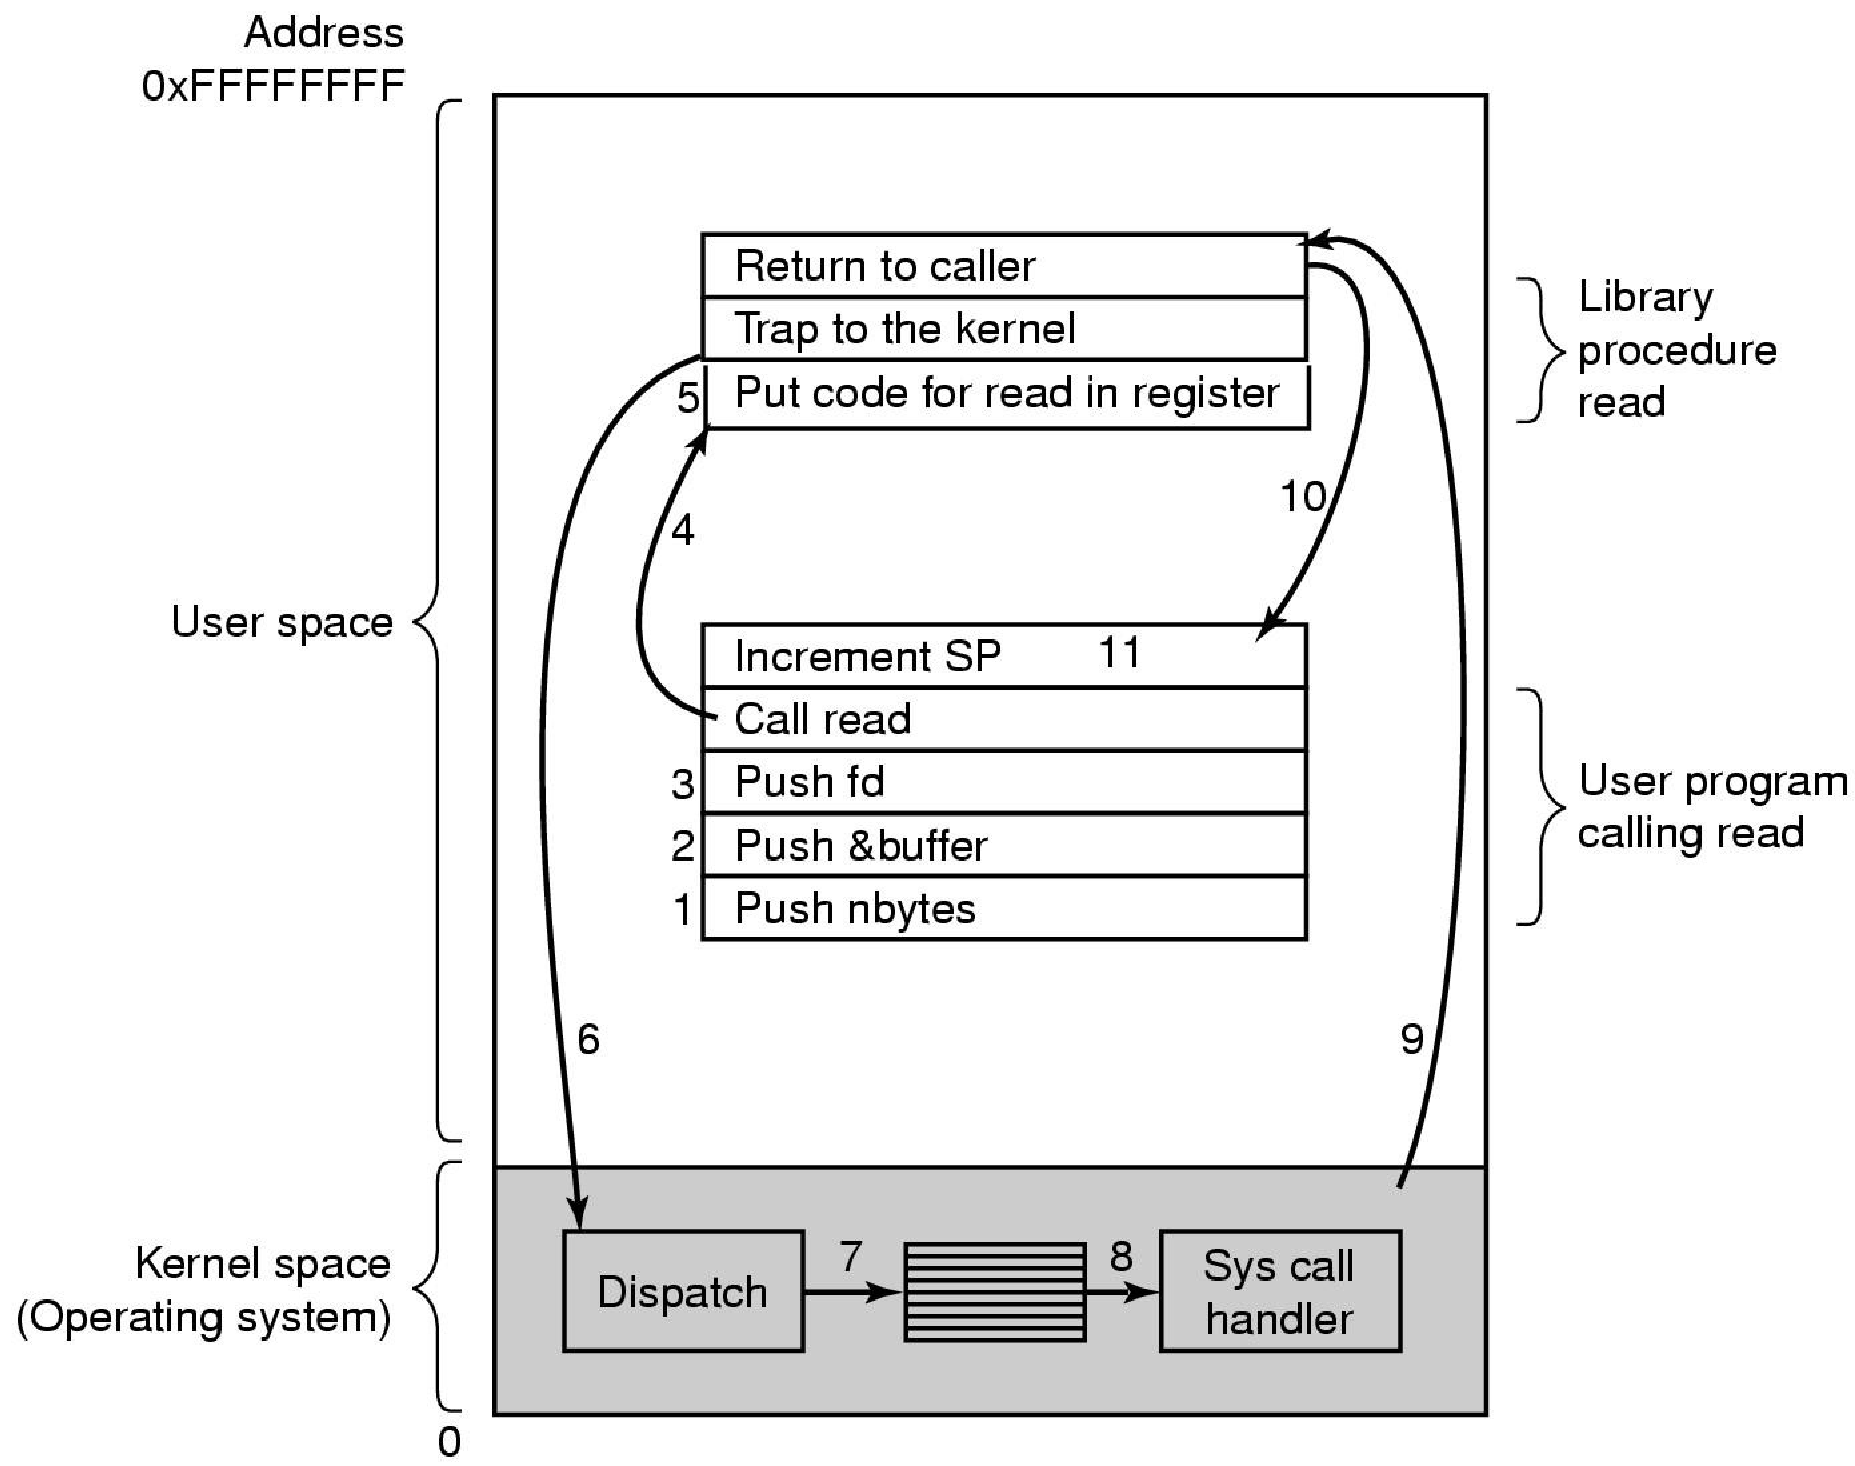
\includegraphics[width=0.7\textwidth]{library_call}
	\caption{Llamado a procedimientos de bibliotecas}
	\label{fig:library_call}
\end{figure}

Referencias de la Figura \ref{fig:library_call}:
\begin{itemize}
	\item 1, 2, 3 y 4 corresponden a un llamado convencional a un procedimiento.
	\item Antes de hacer 5, el sistema operativo habilita el acceso a la memoria del sistema operativo (pasa a modo kernel).
	\item 6 implica una software trap, el procesador pasa a modo protegido.
	\item 7 y 8 se ejecutan en modo protegido del procesador.
	\item En 9 se vuelve a modo usuario del procesador, pero con el sistema operativo en modo kernel.
	\item El paso 10 reestablece la protección de memoria del sistema operativo (sale de modo kernel).
\end{itemize}

\newpage
\section{Procesos}
\subsection{Modelo de procesos}
El sistema operativo debe organizar el software que corre en unidades secuenciales, a esta organización se le llama proceso.\\

Un proceso es:
\begin{itemize}
	\item La imagen de un programa en ejecución (una copia del programa).
	\item Con las estructuras del sistema operativo para administrarlo.
	\item Several processes may be associated with the same program; for example, opening up several instances of the same program often means more than one process is being executed.
\end{itemize}~\\

Un proceso tiene:
\begin{itemize}
	\item La imagen del programa (una copia de su código ejecutable y de su área de datos).
	\item La información acerca de sus estado de ejecución:
	\begin{itemize}
		\item Los valores del program counter, registros y variables.
		\item Información necesaria para su administración por parte del Sistema Operativo (id, prioridad, ...).
	\end{itemize}
	\item Memory (typically some region of virtual memory); which includes the executable code, process-specific data (input and output), a call stack (to keep track of active subroutines and/or other events), and a heap to hold intermediate computation data generated during run time.
	\item Operating system descriptors of resources that are allocated to the process, such as file descriptors (Unix terminology) or handles (Windows), and data sources and sinks.
	\item Security attributes, such as the process owner and the process' set of permissions (allowable operations).
\end{itemize}

Esta información la guarda el sistema operative en estructuras de datos llamadas Process Control Blocks.\\

Any subset of resource, but typically at least the processor state, may be associated with each of the process' threads in operating systems that support threads or 'daughter' processes.

The operating system keeps its processes separated and allocates the resources they need, so that they are less likely to interfere with each other and cause system failures (e.g., deadlock or thrashing). The operating system may also provide mechanisms for inter-process communication to enable processes to interact in safe and predictable ways.

\subsection{Multiprogramación}
In computing, multitasking is a method where multiple tasks (also known as processes) are performed during the same period of time – they are executed concurrently (in overlapping time periods, new tasks starting before others have ended) instead of sequentially (one completing before the next starts). The tasks share common processing resources, such as a CPU and main memory.\\

Multitasking does not necessarily mean that multiple tasks are executing at exactly the same instant. In other words, multitasking does not imply parallelism, but it does mean that more than one task can be part-way through execution at the same time, and more than one task is advancing over a given period of time.

In the case of a computer with a single CPU, only one task is said to be running at any point in time, meaning that the CPU is actively executing instructions for that task.\\

Multitasking solves the problem by scheduling which task may be the one running at any given time, and when another waiting task gets a turn. The act of reassigning a CPU from one task to another one is called a context switch. When context switches occur frequently enough, the illusion of parallelism is achieved.

Even on computers with more than one CPU (called multiprocessor machines) or more than one core in a given CPU (called multicore machines), where more than one task can be executed at a given instant (one per CPU or core), multitasking allows many more tasks to be run than there are CPUs.\\

Cuando hay más de un procesador se conoce como Multiprocesamiento.

Se ejecuta un proceso. Cuando se “bloquea” por I/O, se aprovecha el tiempo para ejecutar otro proceso.

La CPU va conmutando (switching) de un proceso a otro.

Es un multiplexado de la CPU.

\subsubsection{Implementación de la multiprogramación}
El \textit{scheduler} decide a que proceso dar el control.

El \textit{dispatcher} realiza el cambio de estado.

Cada vez que se interrumpe un proceso también se pierde el tiempo de guardar el contexto.

\subsection{Estados de un proceso}
\begin{figure}[H]
	\centering
	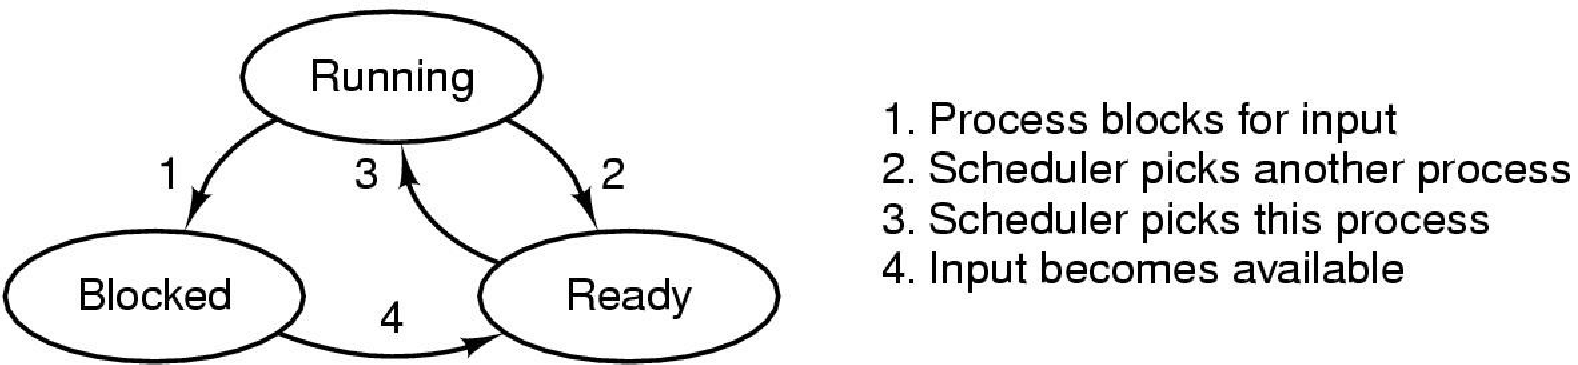
\includegraphics[width=0.7\textwidth]{process_states_simple}
	\caption{Estados de un procedimiento (simplificado)}
	\label{fig:process_states_simple}
\end{figure}

\begin{figure}[H]
	\centering
	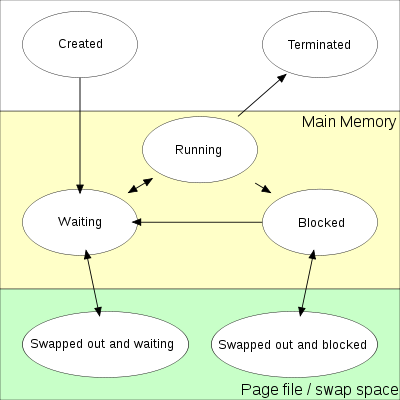
\includegraphics[width=0.5\textwidth]{process_states_full}
	\caption{Estados de un procedimiento}
	\label{fig:process_states_full}
\end{figure}

\subsubsection{Created or New}
When a process is first created, it occupies the ``created'' or ``new'' state. In this state, the process awaits admission to the ``ready'' state. This admission will be approved or delayed by a long-term, or admission, scheduler. Typically in most desktop computer systems, this admission will be approved automatically, however for real-time operating systems this admission may be delayed. In a real time system, admitting too many processes to the "ready" state may lead to oversaturation and over contention for the systems resources, leading to an inability to meet process deadlines.

\subsubsection{Ready and waiting}
A ``ready'' or ``waiting'' process has been loaded into main memory and is awaiting execution on a CPU (to be context switched onto the CPU by the dispatcher, or short-term scheduler). There may be many ``ready'' processes at any one point of the system's execution—for example, in a one-processor system, only one process can be executing at any one time, and all other ``concurrently executing'' processes will be waiting for execution.

A ready queue or run queue is used in computer scheduling. Modern computers are capable of running many different programs or processes at the same time. However, the CPU is only capable of handling one process at a time. Processes that are ready for the CPU are kept in a queue for ``ready'' processes. Other processes that are waiting for an event to occur, such as loading information from a hard drive or waiting on an internet connection, are not in the ready queue.

\subsubsection{Running}
A process moves into the running state when it is chosen for execution. The process's instructions are executed by one of the CPUs (or cores) of the system. There is at most one running process per CPU or core. A process can run in either of the two modes, namely kernel mode or user mode.

\subsubsection{Blocked (Waiting)}
A process that is blocked on some event (such as I/O operation completion or a signal). A process may be blocked due to various reasons such as when a particular process has exhausted the CPU time allocated to it or it is waiting for an event to occur.

\subsubsection{Terminated}
A process may be terminated, either from the ``running'' state by completing its execution or by explicitly being killed. In either of these cases, the process moves to the ``terminated'' state. The underlying program is no longer executing, but the process remains in the process table as a zombie process until its parent process calls the wait system call to read its exit status, at which point the process is removed from the process table, finally ending the process's lifetime. If the parent fails to call wait, this continues to consume the process table entry (concretely the process identifier or PID), and causes a resource leak.\\

A child process always first becomes a zombie before being removed from the resource table. In most cases, under normal system operation zombies are immediately waited on by their parent and then reaped by the system – processes that stay zombies for a long time are generally an error and cause a resource leak.\\

Después de terminado un proceso, el mismo queda en estado ``terminado'' hasta que el sistema operativo termina de limpiar las estructuras que usó para ejecutarlo (mientras tanto está en estado zombie).

% Bibliografía utilizada en el apunte
\newpage
\newcommand{\bibliographyname}{Bibliografía} % Defino el nombre de la sección de la bibliografía
\addcontentsline{toc}{section}{\bibliographyname} % Agrego la bibliografía en el índice
\renewcommand\refname{\bibliographyname} % Renombro a la bibliografía (por default es 'Referencias')
\begin{thebibliography}{X}
	\bibitem{tanenbaum} \textsc{Andrew S. Tanenbaum}, \textit{Sistemas Operativos Modernos}, tercera edición, PEARSON EDUCACIÓN, México, 2009.
\end{thebibliography}

% Incluir los nombres de las personas que han colaborado en la creación del apunte
%\colaborador{Colaborador 1}
%\colaborador{Colaborador 2}
%\revisor{Dr. Profesor}{10/01/2015}
%\makeseccioncolaboradores % Crea la seccion de colaboradres

% Incluir el historial de cambios
\revision{21/02/2012}{Versión inicial con las secciones de Introduccion, Mecanismos básicos.}
%\revision{10/01/2015}{Se agregó una carátula personalizada, una sección con información del proyecto FIUBA Apuntes, la sección de colaboradores del apunte, sección de historial de cambios, ejemplo de bibliografía, ajuste de márgenes, encabezado y pie de página.}
\makehistorial

\end{document}